%!TEX root = ../template.tex
%%%%%%%%%%%%%%%%%%%%%%%%%%%%%%%%%%%%%%%%%%%%%%%%%%%%%%%%%%%%%%%%%%%%
%% chapter2.tex
%% NOVA thesis document file
%%
%% Chapter with the template manual
%%%%%%%%%%%%%%%%%%%%%%%%%%%%%%%%%%%%%%%%%%%%%%%%%%%%%%%%%%%%%%%%%%%%

\typeout{NT FILE chapter2.tex}%

\chapter{Conceitos base e trabalho relacionado}
\label{cha:conceitos_base}

Para obtermos uma melhor percepção do problema descrito no capítulo 1 é necessário perceber em que consiste a visualização de dados, bem como os seus fundamentos e elementos de interação.
Com esse objetivo, neste capítulo, irão ser apresentados os conceitoes bases e o trabalho relacionado que servem de suporte base para o desenvolvimento da tese.

\section{Visualização de Dados}
\label{sec:vis_dados}

%Importância da visualização de dados//Hist´ria e Evolução//Objetivos da Visualização de dados//Desafios na Visualização de dados//Relevância no Contexto Atual

A visualização interativa de dados usa elementos visuais, como diagramas, gráficos ou mapas para representar dados de forma eficiente. Este processo traduz dados complexos, de alto volume em representações visuais, tornado-os mais fáceis de analisar e processar. Através da sua representação visual, é nos permitido identificar padrões, tendências e correlações que de outra forma poderiam passar despercebidos \cite{keim2002information}.

Devido à forma como o ser humano processa e retém informações, o uso de elementos visuais para visualizar grandes quantidades de dados torna se mais eficiente do que relatar toda a informação em relatórios e documentos \cite{ware2019information}. A visualização de dados é uma metodologia simples e rápida de transmitir conceitos de modo universal.
A principal diferença entre visualizações de dados eficazes e ineficazes centraliza-se na capacidade de comunicar a mensagem principal do avaliador de forma clara e direta, sem sobrecarregar a capacidade de memória de trabalho do visualizador \cite{evergreen2013design}.

\subsection{Fundamentos} % (fold)
\label{sub:fundamentos}
                                    %Glossario                                                                                                                                                                                                                                                                                                                                                    ver se aqui é bem esta referencia
A visualização Interativa de Dados (VIS) consiste na representação visual de dados, com o principal objetivo de tranformar dados complexos em formas visuais fáceis de analisar e reter informação. Com o principal objetivo de facilitar a exploração de dados, comunicação e interpretação, este tipo de visualizações desempenham um papel crucial na análise de grandes volumes de informação \cite{keim2002information}.
                                                                                                                        
O design para sistemas de Visualização Interativa de Dados mutas vezes é subdividido em quatro áreas principais. Segundo Tamara Munzner \cite{munzner2014visualization}, essas quatros áreas são: \textit{Domain Situation}, \textit{Data/task abstraction}, \textit{Visual encoding} e \textit{Algorithm}. Cada uma destas áreas desempenha um papel crucial na implementação do design de sistemas de visualização de dados. Como é possível observar na figura \ref{fig:tamara-munzner-principles}, o gráfico serve como guia para criar visualizações de dados de uma forma eficaz e eficiente. Este apresenta uma estrutura concêntrica, onde cada nível do design depende do nível anterior.

\begin{figure}[htbp]
  \centering
  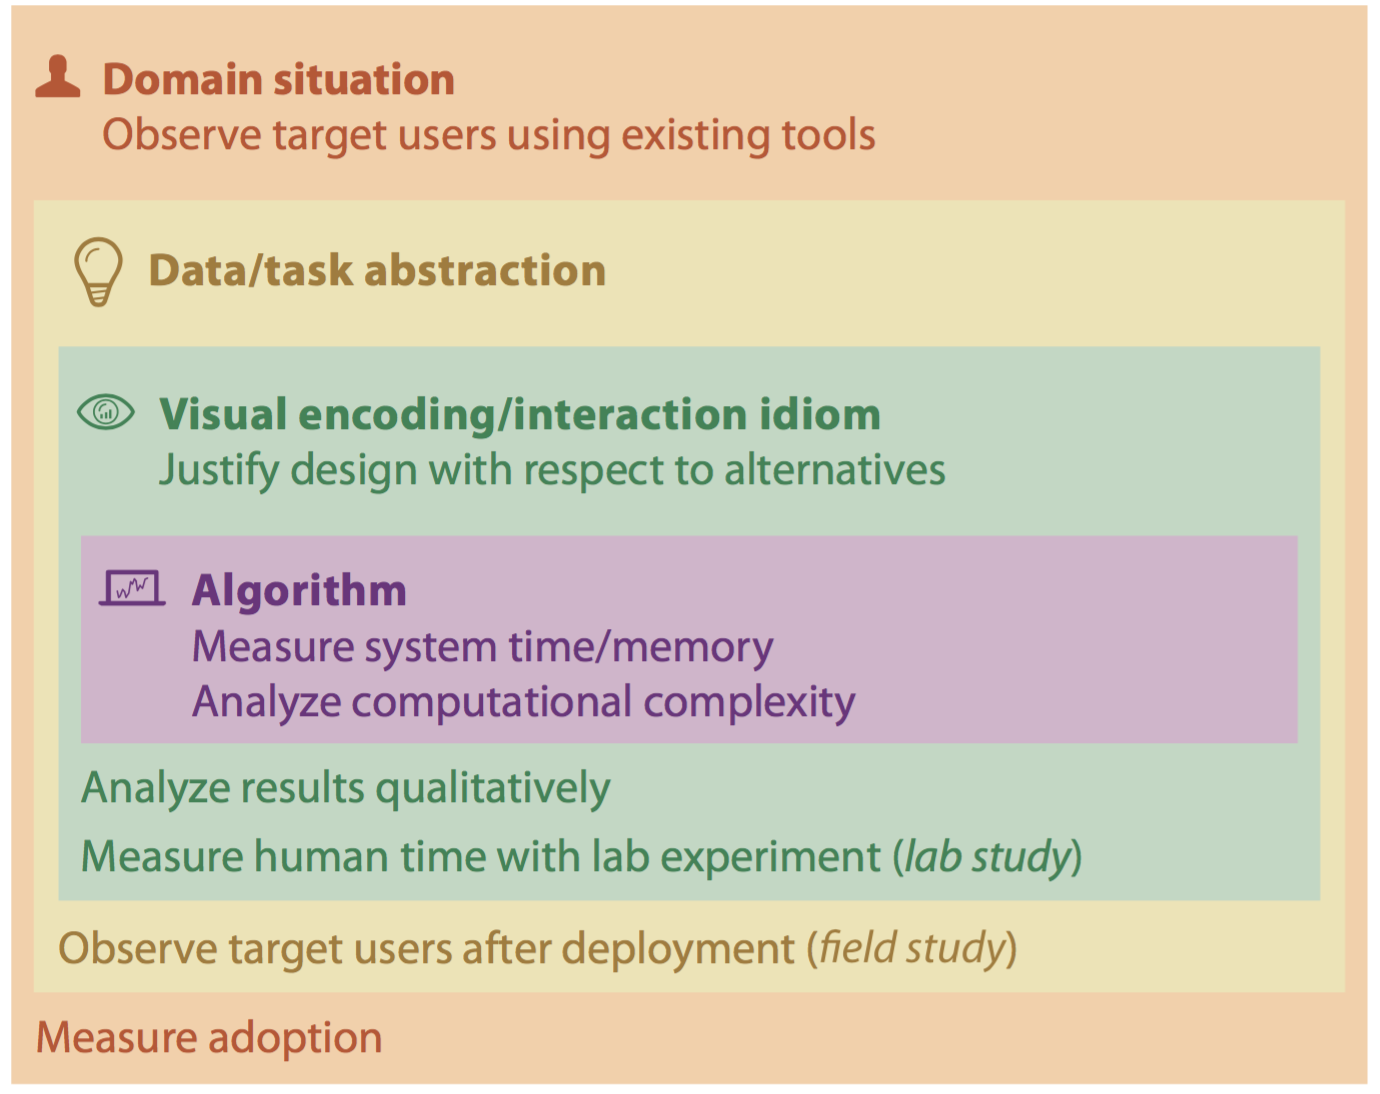
\includegraphics[height=3in]{tamara-munzner2}
  \caption{Exemplo dos 4 níveis de design para sistemas de visualização de interativa de dados.}
  \label{fig:tamara-munzner-principles}
\end{figure}

O primeiro nível apresentado no gráfico da figura \ref{fig:tamara-munzner-principles} é o \textit{Domain Situation}. Este nível representa o ponto de partida inicial do processo de design de visualizações, onde se realiza a análise do contexto no qual a visualização irá ser utilizada. O foco principal deste nível está nos \textit{stakeholders}, é para estes utilizadores que a visualização é direcionada.
Para garantirmos a maior eficácia da visualização, precisamos de garantir que esta está alinhada aos interesses dos utilizadores. Para isso, é imperativo compreender quem são os utilizadores-alvo, quais as suas necessidades, e como é que os mesmo interagem com os dados e ferramentas disponívies \cite{courage2005understanding}.

O segundo nível do modelo é o nível que traça a ponte entre a compreensão do domínio e o design concreto da visualização, mantendo como foco principal a abstração dos dados e tarefas  do contexto específico. Este nível tem como objetivo transformar as necessidades e questões dos \textit{stakeholders}, identificadas no nível superior, em abstrações concretas que possam ser resolvidas através de visualizações de dados, para isso, os dados e as intenções dos utilizadores são filtradas e hierarquizadas, de forma a criar uma base para as decisões de design visual. 
É através destas técnicas e metodologias de filtragem de interesses e questões que é definida de forma clara a estrutura e conteúdo da visualização, ou seja, a que questões a visualização vai responder, e com que dados o fará. Um design bem alcaçado depende diretamente da qualidade da abstração dos dados e tarefas obtidas neste nível.

O terceiro nível do modelo, \textit{Visual Encoding/interaction idiom}, é o nível onde os dados e tarefas abstraídas do processo aplicado no nível anterior são transformados em representações visuais interativas. Este nível define a estrutura e organização dos dados a serem representados visualmente, bem como a forma como os utilizadores podem interargir com os mesmos.
A codificação visual é uma técnica focada na representação dos dados, através de propriedades visuais, como posição, cor e tamanho. A escolha dos elementos visuais a utilizar e como os mesmos são organizados são a chave para uma visualização bem sucedida, evitando assim sobrecarregar os utilizadores com designs complexos e confusos.
Os idiomas de interação como o nome indica, são os elementos usados na visualização que permitem aos utilizadores interargir diretamente com a visualização. Estes idiomas incluiem elementos como filtragem, zoom, tooltip e highlight de elementos. Estas interações tornam a visualização mais dinãmica, uma vez que permitem a direta interação com os componentes, facilitando a exploração e análise dos dados \cite{figueiras2015towards}.
Este nível estabelece uma ligação direta entre os dados abstraídos do nível anterior \textit{Data/task abstraction} aos algoritmos necessários para implementar as interações no nível seguinte \textit{Algorithm}. Um design simples, de fácil utilização e percepção, é essencial para criar visualizações intuitivas, ao passo que uma abordagem complexa e de difícil percepção neste nível pode resultar em visualizações confusas e pouco eficazes.

O último nível do diagrama da figura \ref{fig:tamara-munzner-principles}, foca na implementação técnica das visualizações através do desenvolvimento de algoritmos e técnicas de interação. Este nível junta todas as escolhas feitas dos níveis anteriores, tranformando-as em processos computacionais que permitam as visualizações e interações serem executadas corretamente.

%\subsection{Elementos de interação na Visualização de Dados}
\subsection{Interação na Visualização de Dados} % (fold)  
\label{sub:elem_int}

Com o constante progresso da ciência, estudos mostram que os humanos são mais propicios de captar informação quando interagem diretamente com a mesma através de filtragens e destaques face à simples interação com visualizações estáticas \cite{heer2012interactive}. 

Os sistemas de \textit{Information Visualization (InfoVis)} são compostos essencialmente por duas componentes principais: representação e interação. A componente de representação é centrada na representação gráfica computacional dos elementos e onde os mesmo se vão situar no \textit{display}. A componente de interação é relatada como o dialogo entre o utilizador e o sistema enquanto o utilizador explora padrões e relações nos dados exibidos \cite{yi2007toward}. 

Apesar destas componentes seram definidas em separado, as mesmas estão interligadas, dependendo uma da outra. A interação desempenha um papel crucial na visualiação de informação. A omissão da componente interativa num sistema \textit{InfoVis} resulta numa visualização estática. Este tipo de visualizações estática tornam-se mais limitadas com o aumento de informação a ser disponibilizada.

A forma como interagimos com os dados nem sempre depende da técnologia utilizada, mas da maneira como o nosso cérebro processa informação. O cérebro humano processa imagens e interações visuais de forma mais rápida e informativa em comparação com texto ou informação isolada \cite{ware2019information}.

Segundo John Sweller, o modelo da carga cognitiva revela que quando um utilizador é exposto a uma grande quantidade de informação, o cérebro tem dificuldade em processar e reter a toda a informação disponibilizada, causando uma sobrecarga cognitiva \cite{sweller1988cognitive}. Para evitar este tipo de sobrecarga, elementos interativos como filtragem, destaque e drill-down dão a possibilidade aos utilizadores de explorar os dados de forma gradual, reduzindo assim a complexidade de informação apresentada.

A maneira como os utilizadores interagem com as visualizações é dividida em dois modelos cognitivos: exploração livre e interpretação guiada.

Com base nestes dois processos cognitivos, a visualização de dados pode ser considerada exploratória ou explicativa. A visualização exploratória é uma abordagem que foca na descoberta e análise dos dados por parte do utilizador. O utilizador tem a possibilidade de interargir de forma livre com os dados procurando erros, insights, e padrões presente nos dados. A visualização explicativa tem uma abordagem mais rígida e estática, limitando as interações que o utilizador pode tomar consuante a visualização apresentada. Esta abordagem é mais comum em visualizações que já se encontram implementadas para guiar o utilizador a uma conclusão ou resultado específico \cite{heer2012interactive}. 

Ao abrangir a área de interação na visualização de dados, somos por vezes deparados com desafios e limitações nas visualizações de dados. Ao aumentarmos o conjunto de elementos interativos numa visualização, não implica necessáriamente que a mesma melhore a sua qualidade. Por vezes, este aumento de elementos apenas sobrecarga cognitivamente os utilizadores, dificultando a navegação na mesma. Aumentar a qualidade de interação numa visualização implica melhorar a qualidade dos elementos interativos, tendo em análise o contexto inserido, priorizando sempre a interação dos utilizadores com as técnologias usadas e tendo em conta o leque de perfis que os utilizadores alvo podem ter. Este cuidado aumenta o desempenho cognitivo do utilizador, promovendo a usabilidade e compatibilidade no contexto inserido \cite{dimara2019interaction}. 

% em cima falei de como podemos contornar as limitações melhornado a interação, ou seja antes posso explorar cada limitação mais detalhadamente

\subsection{Taxonomias de interação} % (fold)
\label{sub:taxonomias_interacao}

%abstract do Yi como introdutorio faz a separação da interação (capitulo anterior) com taxonomias de interação
%Yi- refere qual é que e o grande desafio da interação (vermelho)
%Figueiras - referencia de YI no texto de Figueiras (vermelho)
Apesar da interação apresentar um papel importante nos sistemas de visualização de dados, tem vindo a receber pouca atenção na comunidade \textit{InfoVis}. Poucas \textit{frameworks} e taxonomias de interação existem sendo que, as existentes tipicamente centralizam-se em tarefas abstratas de alto nível, não se preocupando com os benfícios que a interação nos sistemas de visualização de dados pode trazer. Segundo Foley e outros, as técnicas de interação são muitas vezes definidas pela forma como os dispositivos físicos de entrada e saída são usados para resolver tarefas de diálogo entre os humanos e computadores \cite{foley1996computer}. No entanto, no contexto dos sistemas \textit{InfoVis}, as técnicas de interação são defendidas como sendo mais apropriadas no que toca a sua capacidade de modificar, ajustar ou criar representações visuais. A implementação e definição de taxonomias de interação é crucial para a compreensão e desenvolvimento de sistemas de visualização de dados. No entando, segundo Yi e outros, definir uma taxonomia é algo desafiante uma vez que a mesmo se pode tornar obsoleta se uma nova técnica de interação que não se enquadre na taxonomia definida for descoberta.

Desta forma, após a extensa revisão dos sistemas \textit{InfoVis} e das suas técnicas de interação, estudos foram realizados sobre as propostas de taxonomias de interação. Segundo Ana Figueiras, para que seja possível estudar o impacto que a interatividade tem nos sistemas \textit{InfoVis}, é necessáro estudarmos e analisarmos as técnicas de interação que podem ser impostas nestes tipos de visualização, levando-nos à conslusão que muitas das taxonomias existentes não englobam técnicas de interação novas como é o exemplo da \textbf{gamificação} \cite{figueiras2015towards}. Ao analisar as taxonomias propostas por Yi et al., D.A. Keim  e Ben Shneiderman, Ana propôs 11 categorias de interação que englobam as técnicas mais usadas por este tipo de sistemas:

%Desta forma, após a extensa revisão dos sistemas \textit{InfoVis} e das suas técnicas de interação, Yi e outros propuseram 7 categorias de interação que englobam as técnicas mais usadas por este tipo de sistemas \cite{yi2007toward}:

\begin{itemize}
  \item \textbf{Seleção}: Selecionar dados de interesse.
  \item \textbf{Exploração}: Explorar os dados.
  \item \textbf{Reconfiguração}: Mudar a organização da informação disponibilizada.
  \item \textbf{Codificação}: Mostrar uma representação diferente.
  \item \textbf{Abstração/Elaboração}: Ajustar o nível de detalhe.
  \item \textbf{Filtro}: Mostrar algo segundo uma condição.
  \item \textbf{Conexão}: Mostrar dados relacionados.
  \item \textbf{Histórico}: Possibilidade de retornar ações. %shneiderman
  \item \textbf{Extração de funcionalidades}: Extrair dados de interesse. %shneiderman
  \item \textbf{Participação/Colaboração}: Contribuição dos utilizadores nos dados.
  \item \textbf{Gamificação}: Mostrar informação de uma forma mais lúdica.
\end{itemize}

As técicas de \textbf{Seleção} são técnicas que permitem aos utilizadores selecionar diferentes conjuntos de dados de maior interesse de forma a conseguir monitorizá-los e mantê-los sob vigilância. Este tipo de técnicas são muitas vezes usadas para auxiliar a cognição dos utilizadores. Ao ser possível manter sob vigia os diferentes items ou conjuntos de dados selecionado pelo utilizaodr, no caso de a informação sofrer constantes alterações nas suas representações visuais ou diretamente no conjunto de dados, o utilizador consegue facilmente identificar as alterações efetuados e manter-se atualizado sobre a informação que lhe é relevante \cite{yi2007toward, figueiras2015towards}.

Nos sistemas \textit{InfoVis}, devido a limitações impostas pelo tamanho dos ecrãs para mostar informação, ou pelas limitações de processamento cognitivo por parte dos humano ao processar os dados que estão, os criadores de visualizações por vezes optam por mostrar apenas um número limitado de elementos visuais por visualização. As técnicas de \textbf{Exploração} ultrapassam estas limtações, dando a possibilidade de os utilizadores explorarem os diferentes conjuntos de dados. Das principais técnicas utilizadas nesta categoria de interação destaca-se o \textit{panning}, que é definido como o movimento de uma câmera digital numa cena, sendo por vezes simulado este efeito com o uso de \textit{scroll-bars}. 

A \textbf{Reconfiguração} é uma técnica que por vezes é também utilizada na categoria de \textbf{Exploração}. É através desta técnica que os utilizadores têm a possibilidade de alterar a disposição espacial dos dados obtendo novas perspetivas sobre a informação disponibilizada \cite{yi2007toward, figueiras2015towards}.

Por vezes, as representações visuais com o mesmo tipo de dados podem ser codificadas de forma diferente. Este tipo de \textbf{Codificação} é uma técnica que permite aos utiilizadores alterarem a forma visual como os dados são representados. Estas alterações podem ocorrer a nível das cores, tamanho, ou até na forma como os dados são apresentados. É através da alteração destes elementos visuais que os utilizadores obtêm diferentes perspetivas sobre os dados, facilitando a identificação de relacações entre os diferentes conjuntos de dados \cite{yi2007toward}.

Várias técnicas de \textbf{Abstração/Elaboração} são usadas nos sistemas \textit{InfoVis}. Estes tipos de interação oferecem aos utilizadores a possibilidade de ajustar o nível de detalhe nas visualizações apresentadas de acordo com os seus interesses pessoais e objetivos de visualização \cite{yi2007toward, figueiras2015towards}. A técnica de \textit{Zooming} é um exemplo muito comum e bastante utilizado neste contexto. Esta técnica age como um tipo de filtro por navegação, aumentando o nível de detalhe dos elementos selecionados ao mesmo tempo que remove os elementos menos relevantes do plano, mantendo o foco apenas nos elementos selecionados de maior interesse. O uso desta técnica facilita duas tarefas cognitivas em visualizações. Ao efetuar \textit{zoom-in} os utilizadores são deparados com a organização de informações de forma mais detalhada e estruturada deixando de fora elementos externos de menor interesse. Ao efetuar \textit{zoom-out} é possível visualizar informações que estavam inicialmente escondidas ou das quais os utilizadores não se recordava. \textit{Details-on-demand} é outra técnica de interação muito comum nesta categoria. Um exemplo das técnicas mais comuns nas operações \textit{details-on-demand} são as técnias de \textit{drill-down} e \textit{tooltips/popups}. As técnicas de \textit{drill-down} são muito comuns em visualizações \textit{treemap}, uma vez que é possível visualizar apenas os níveis e sub-níveis de maior interesse. Esta técnica permite que as limitações de ecrã e complexidade visual sejam tratadas, mantendo uma representação geral dos dados. As técnicas de \textit{tooltips/popups}, muitas vezes acionadas ao efetuar \textit{hover} ou \textit{click} sobre determinado elemento na visualização, mostram ao utilizador informações adicionais sobre os elementos em análise \cite{figueiras2015towards}.

As técnicas utilizadas na categoria de \textbf{Filtro} permitem aos utilizadores mudar o conjunto de dados apresentado consuante condições específicas impostas pelos mesmos, desta forma toda a informação que não cumpra as condições impostas é removida da visualização. Esta forma simplificada de filtrar a informação disponibilizada deixando de parte os elementos de menor interesse é uma forma de reduzir a carga cognitiva dos utilizadores, permitindo-lhes focar apenas no que lhes é relevante visualizar. As implementações destas técnicas requerem uma resposta por parte do sistema imediata, caso contrário, pode afetar negativamente não só experiência do utilizador na visualização como a interpretação dos dados pode ser comprometida. Este tipo de técnicas podem ser enquadradas nas técnicas de seleção, uma vez que possuem características semelhantes ao destacar apenas os elementos de maior interesse durante a sua visualização \cite{figueiras2015towards, yi2007toward}.

\textbf{Conexão}, ou relacionamento, é a categoria de interação que permite o utilizador visualizar as relações entre os diferentes conjuntos de dados. Este tipo de relação é muitas vezes mostrado através de técnicas como \textit{highlight} onde são destacados os conjuntos de dados que se encontram relacinados com os dados selecionados pelo utilizador. Este tipo de técnicas usadas para distinguir os diferentes conjuntos de dados diminuem a carga cognitiva imposta sobre os utilizadores. Caso este tipo de técnicas de relacionamento não tivessem a capacidade de dar \textit{highlight} nos elementos de maior interesse, seria bastante complicado para o utilizador efetuar comparações devido ao elevado ruído visual imposto pelas visualizações \cite{figueiras2015towards}.

Segundo Shneiderman, a exploração de informação é um processo longo que envolve bastantes passos para a sua análise, desta forma, manter o \textbf{Histórico} das ações efetuadas pelos utilizadores e permitir aos mesmo refazer as suas ações é crucial \cite{heer2012interactive}. Dar a possibilidade de o utilizador efetuar ações como \textit{undo} e \textit{replay} permite não só a recuperação de erros que possam surgir na exploração de informação como progressivamente melhorar a sua análise dos dados. Este tipo de técnicas são muitas vezes desconsideradas e esquecidas no que toca a implementação de sistemas \textit{InfoVis} \cite{figueiras2015towards}. Outra técnica menos comum é a \textbf{Extração de funcionalidades}. Explorar os dados por vezes pode ser uma tarefa longa e complexa, desta forma, dar a possibilidade de os utilizadores extrairem informação para a mesma ser compartilhada, repartida ou até visualizada com outras visualizações pode reduzir a complexidade da análise dos dados \cite{figueiras2015towards, heer2012interactive}.

Técnicas como \textbf{Participação/Colaboração} são técnicas que envolvem a direta contribuição dos utilizadores nos dados apre sentados de forma a facilitar a sua interpretação e perceção. Por vezes este tipo de técnicas não chegam a ser implementados devido ao consumo de tempo que a mesma pode tomar \cite{figueiras2015towards}. 

Por fim, a \textbf{Gamificação} é considerada uma das técnicas interativas mais complexas de adicionar num sistema \textit{InfoVis}. Segundo Deterding \cite{deterding2011game}, gamificação pode ser brevemente definida como o uso de elementos de design de jogos em contextos não relacionados com jogos. Apesar de ser uma técnica cuja implementação por vezes é bastante demorada e complexa, esta contém uma panoplia de elementos como contextos narrativos, recompensas, \textit{ranks}, nívels e objetivos de forma a tornarem a experiência do utilizador mais lúdica e cativante, contrariando as práticas comuns que por vezes podem passar por serem monótonas e aborrecidas \cite{figueiras2015towards}.

\section{Design de \textit{Dashboard}}
\label{sec:design_dashboard}
%Capitulo 3 de "Riding the Technology Wave" pode aprofundar a introdução
%Os \textit{dashboards} com o passar dos anos têm vindo a ser cada vez mais requisitados no que toca a visualização de dados \cite{sarikaya2018we}. Este tipo de ferramente oferece aos utilizadores a posssibilidade de não só visualizar, como interagir com a informação disponibilizada, facilitando a compreensão e interpretação da informação disponibilizada.

Com o passar dos anos, o uso de \textit{dashboards} tem vindo a ser uma técnica cada vez mais comum no que toca visualização de informação \cite{sarikaya2018we}. 

Num contexto empresarial, o termo "\textit{dashboard}" é usado para descrever um sistema que visualiza informação útil para a tomada de decisões \cite{janes2013effective}. Segundo Few, um \textit{dashboard} é uma representação visual da informação mais importante do conjunto de dados, necessária para atingir um determinado objetivo, consolidadas e ordenadas num único ecrã de forma à informação ser monitorizada num instante \cite{few2005common}. O design deste tipo de ferramenta tem uma enorme influência no \textit{outcome} dos resultados e interações esperadas por parte dos utilizadores. 

Com o constante crescimento do volumes de dados, o uso de \textit{dashboards} para a análise e tomada de decisões tem vindo a ser cada vez mais usado. No entanto, a implementação deste tipo de ferramentas é considerada uma tarefa complexa e por vezes incerta. O design deste tipo de ferramentas tem de ser direcionado ao público-alvo pelo qual estamos a considerar, tendo em conta as suas necessidades, sem sobrecarregar o utilizador com informação desnecessária e irrelevante para o contexto inserido. O mau design deste tipo de ferramentas pode muitas vezes levar à má interpretação dos dados por parte do utilizador.

De forma a que o design da \textit{dashboard} se encontre enquadrada com as necessidades do utilizador, é necessário que num primeiro cenário se conheça o público-alvo, ou seja, os seus objetivos com a visualização, e as respostas que pretendem ver respondidas. Para este design se alinhar com os objetivos impostos, definir métricas como que visualizações utilizar, e que técnicas de interação implementar, são fatores chave para o sucesso da visualização. Uma \textit{dashboard} que cumpra os objetivos impostos pelo utilizador, é uma \textit{dashboard} que é visualizada sem sobrecarregar os utilizadores, esclarecendo todos as questões impostas pelos mesmos \cite{pappas2011riding}. Desta forma podemos usar um modelo chamado \textit{Goal-Questio-Metric}. Este modelo é uma abordagem direcionada para a definição de objetivos através da definição de questões e métricas que iram ser necessárias para aringir os objetivos propostos \cite{janes2013effective}. Este modelo é composto por 3 níveis como é mostrado na figura \ref{fig:gqm-model}.

\begin{itemize}
  \item Nível Conceptual: Define os \textbf{objetivos} que se pretendem atingir tendo em conta questões como "O que é que se pretende alcançar com a visualização?".
  \item Nível Operacional: Define as \textbf{questões} que são necessárias para averiguar quais os aspetos relevantes para atingir os objetivos propostos. 
  \item Nível Quantitativo: Dtermina as \textbf{medidas} que definem que dados iram ser utilizados para responder às questões propostas.
\end{itemize}

\begin{figure}[htbp]
  \centering
  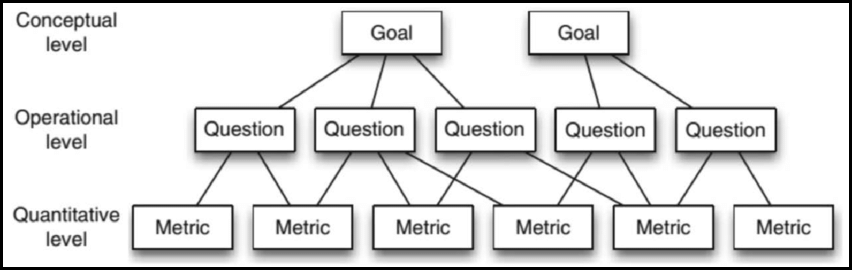
\includegraphics[height=1.5in]{GQM-model-structure2}
  \caption{Estrutura do modelo GQM \cite{article}.}
  \label{fig:gqm-model}
\end{figure}

\subsection{Desafios no Design de \textit{Dashboards}}
\label{sec:desafios_design}

Muitas vezes, os \textit{dashboards} são desenhados segundo más práticas de design, onde o intuito principal é mostrar o maior número de visualizações dos dados possíveis. Este tipo de abordagem apenas serve para mostrar as capacidades gráficas do sistema, de forma a impressionar futuros utilizadores, em vez de se focar no principal objetivo deste tipo de ferramenta, a representação clara de informação \cite{janes2013effective}. Muitos dos desafios e limitações que são impostos na implementação dos \textit{dashboards} surgem devido a fatores externos, como a performance e o tempo de resposta do sistema, ou fatores internos, como a escolha errada de elementos visuais. 

As restrições tecnológicas muitas vezes limitam o desempenho e a performance das \textit{dashboards}. A escolha de elementos de interação com uma complexidade e peso elevados podem levar a um mau desempenho, a nível da performance e tempo de resposta do sistema, tornando a experiência do utilizador por vezes frustrante e pouco apelativa \cite{eckerson2010performance}. 

A nível da usabilidade e acessibilidade, por vezes os designs não engloblam nem consideram a diversidade de perfis que o sistema pode ter, apenas se focando num "utilizador-tipo", o que por vezes pode levar a um esforço acrescido por parte dos utilizadores ao analisar o conteúdo das visualizações. Uma solução para contornar este comportamento é dar a possibilidade de criar \textit{dashboards} com diferentes níveis de complexidade e personalização. Além disto, muitos \textit{dashboards} hoje em dia falham na consideração de diferentes tipos de deficiências que os utilizadores possam ter, como é o que caso das pessoas daltónicas. Ao englobar diferentes tipos de deficiências no design das \textit{dashboards}, é possível criar um ambiente mais inclusivo e acessível para todos os utilizadores.

Ao nível da comunicação, as \textit{dashboards} que comunicam com os utilizadores de forma clara, concisa, e eficiente, são o resultado de um design cuidado e informativo \cite{few2005common}. A clareza com que a informação é apresentada aos utilizadores é crucial para um design eficiente. Erros relacionados com a organização e exibição dos dados levam muitas vezes à má interpretação da informação por parte dos utilizadores. A má comunicação do \textit{dashboard} pode surgir quando o design da mesma não está orientado para o publico-alvo em questão, tornando a sua interpretação mais complexa e duradora.

Ao nível da interatividade, esta surge grande parte das vezes através do uso de técnicas de interação mais comuns, como é o caso do teclado e rato, em vez de tomarem vantagem das diferentes formas de interação possíveis neste tipo de sistemas. A falta de interação, ou a interação excessiva, são fatores que afetam diretamente a forma como os utilizadores percecionam a informação. A introdução de elementos interativos nos \textit{dashboards} aumentam a retenção de informação por parte dos utilizadores \cite{heer2012interactive}. No entanto, a implementação de técnicas com uma interações excessiva e complexa podem levar a uma sobrecarga cognitiva por parte dos utilizadores, dificultando a sua interpretação dos dados.

%Por fim, ao nível da interatividade, o uso de elementos físicos como o rato e o teclado tornam-se os meios de interação mais comuns, em vez de tomarem vantagem das diferentes formas de interação possíveis neste tipo de sistemas. A interação excessiva , ou por vezes a falta de interação, são fatores que prejudicam a forma como os utilizadores interagem e percecionam a informação mostrada. Com a introdução de diferentes elementos interativos nos \textit{dashboards}, a retenção de informação por parte dos utilizadores aumenta \cite{heer2012interactive}. No entanto, a implementação de técnicas de interação excessivas e complexas pode levar a uma sobrecarga cognitiva dos utilizadores, dificultando a sua interpretação dos dados.

\subsection{Tipos de Dashboards} % (fold)
\label{sub:tipos_dashboards}
%Ver documentos de Ikechukwu et al. (2012) & Few (2006), sobre os diferentes tipos de dashboards (operacionais, estratégicos, analíticos)
%estrutura: introdução(2.Data Dashboard Categories-Riding the Technology), listar os tipos de dashboards, falar sobre cada um em detalhe(Riding the Technology//What do we talk about)
De forma a uma \textit{dashboard} ser considerada uma ferramenta útil para a visualização de informação, é necessário apresentar a informação de forma eficaz, e dar ao utilizador a possibilidade de interagir de forma direta e natural com a informação apresentada. Desta forma, para alcançar este nível de eficácia numa visualização, determinar parâmetros como o público-alvo e o objetivo da visualização são fundamentais \cite{pappas2011riding}.

\textit{Dashboards} que apoiam esta tomada de decisão podem ser divididos em três categorias:

\begin{itemize}
  \item \textbf{Estratégicos}: ~\ref{fig:strat-dash}
  \item \textbf{Operacionais}: ~\ref{fig:op-dash}
  \item \textbf{Analíticos}: ~\ref{fig:anal-dash}
\end{itemize}

Os \textit{dashboards} estratégicas são \textit{dashbords} que reportam aos diferentes departamentes de uma organização qual a situação geral de uma empresa. A representação neste tipo de \textit{dashboards} é de alto nível, focando-se nos diferentes \textit{KPIs} e métricas de negócio a longo prazo. Ao apresentarem uma representação alto nível, este tipo de \textit{dashboards} não possuem visualizações que entrem em detalhe sobre os dados apresentados, agregando os diferentes dados apresentados de forma a criar uma visualização global sobre a situação atual da organização. Ao apresentarem uma janela temporal bastante alargada, o design deste tipo de \textit{dashboards} ter de ser claro e bem estruturado, de forma a facilitar a interpretação dos dados por parte dos seus utilizadores \cite{pappas2011riding}. 

Os \textit{dashboards} operacionais, de forma semelhante aos \textit{dashboards} estratégicos, necessitam de ter um design simples e organizado de forma a que os seus utilizadores possam, através da rápida visualização da informação disponibilizada, identificar medidas e métricas que se encontrem fora dos limites normais definidos pela organização, necessitando uma intervenção imediata \cite{pappas2011riding}. Este tipo de \textit{dashboards}, em comparação com os \textit{dashboards} estratégicos, necessitam de um nível mais detalhado e atualizado de informação, uma vez que a principal função deste tipo de \textit{dashboards} é controlar, e monitorizar as operações e processos envolventes numa organização em tempo real. Ao necessitar de uma quantidade elevada de informação em tempo real, \textit{performance} é uma característica crucial neste tipo de visualizações, uma vez que, com o constante fluxo de informação, se o design for algo complexo e pouco eficiente, a interpretação da informação pode ficar comprometida, atrasando a tomada de decisão dos utilizadores, o que pode comprometer o funcionamente da organização.

Os \textit{dashboards} analíticos partilham atributos comuns com os \textit{dashboards} estratégicos e operacionais, uma vez que podem apresentar informação consuante um grande espaço temporal como as \textit{dashboards} estratégicas, e informação detalhada como as \textit{dashboards} operacionais. No entando, o principal propósito deste tipo de \textit{dashbaord} é a decoberta de padrões e tendências nos dados, através da constante interação e exploração de informação, consuante diferentes janelas temporais.

Em relação ao nível de interatividade que cada tipo de \textit{dashboards} necessita de ter, este varia de forma crescente consuante as categorias mencionadas. Os \textit{dashboards} estratégicos uma vez que apresentam uma visão geral da organização, num espaço temporal alargado não necessitam de ter um nível de interatividade elevado. As \textit{dashboards} operacionais necessitam de apresentar um nível de interação mais moderado, desta forma, é possível monitorizar as operações da organização em tempo real. O tipo de \textit{dashboard} que necessita de ter um nível de interativadade mais elevado são as \textit{dashboards} analíticas. Este tipo de dashboards ao apresentarem diferentes janelas temporais, e com o principal objetivo de encontrar tendências e padrões nos dados, é crucial que nas suas visualizações estejam incorporados elementos de interação como \textit{drill-down}, \textit{filtering} e \textit{highlighting}, de forma a facilitar a navegação do utilizador pela \textit{dashboard}.

\begin{figure}[htbp]
  \begin{subfigure}{0.5\textwidth}
    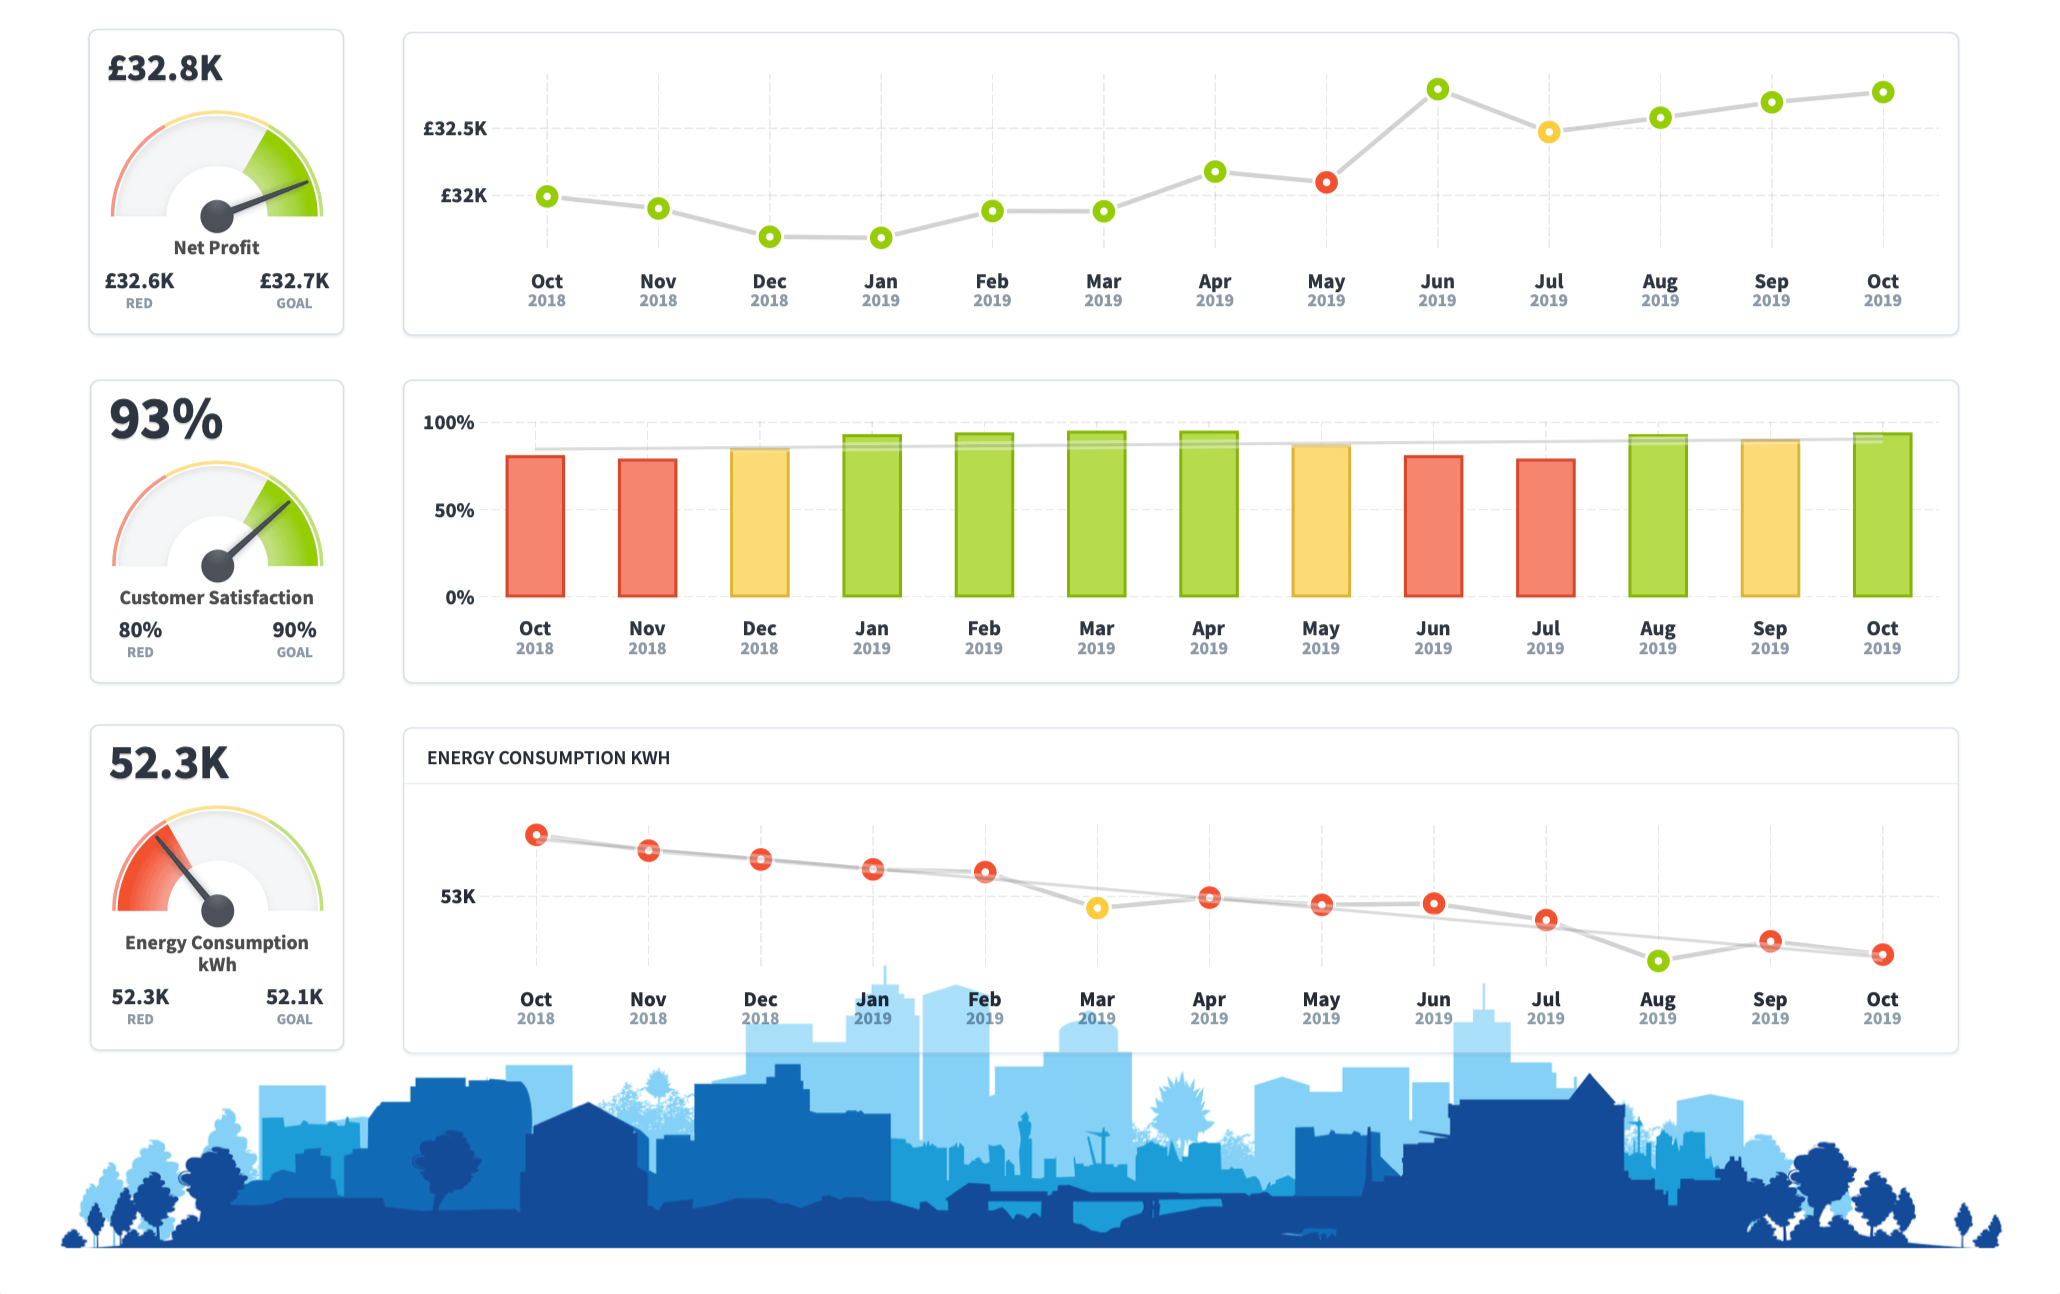
\includegraphics[width=0.9\linewidth, height=5cm]{strategic-dashboard.png} 
    \caption{Exemplo de um \textit{dashboard} estratégico}
    \label{fig:strat-dash}
  \end{subfigure}
  \begin{subfigure}{0.5\textwidth}
    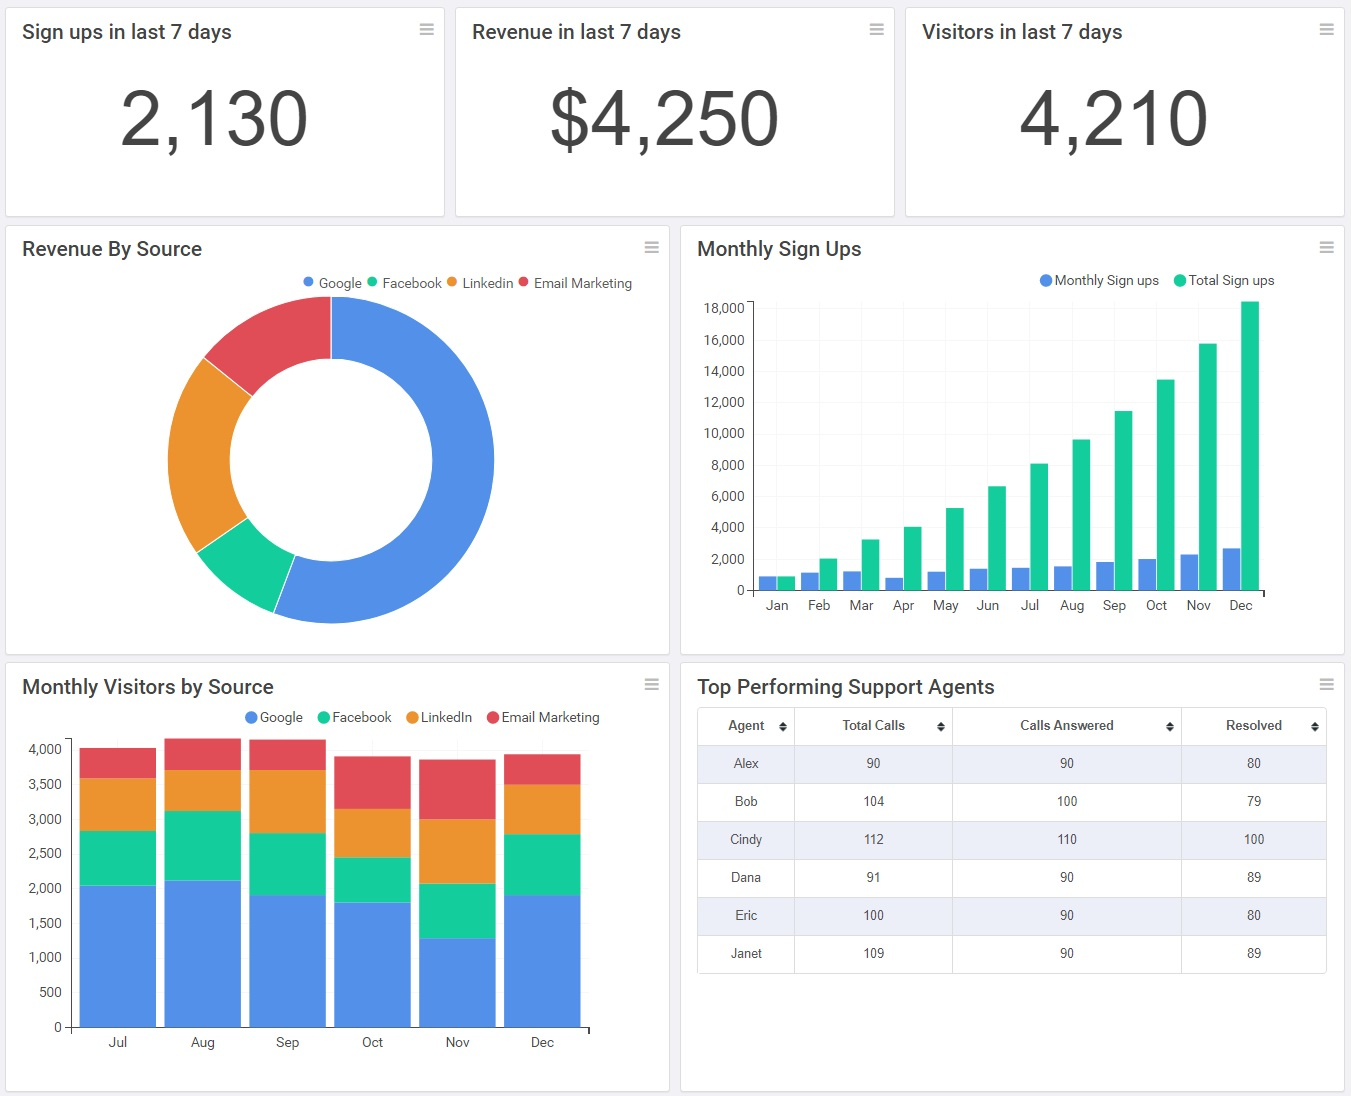
\includegraphics[width=0.9\linewidth, height=5cm]{operational-dashboard.jpg}
    \caption{Exemplo de um \textit{dashboard} operacional}
    \label{fig:op-dash}
  \end{subfigure}
  \begin{subfigure}{0.5\textwidth}
    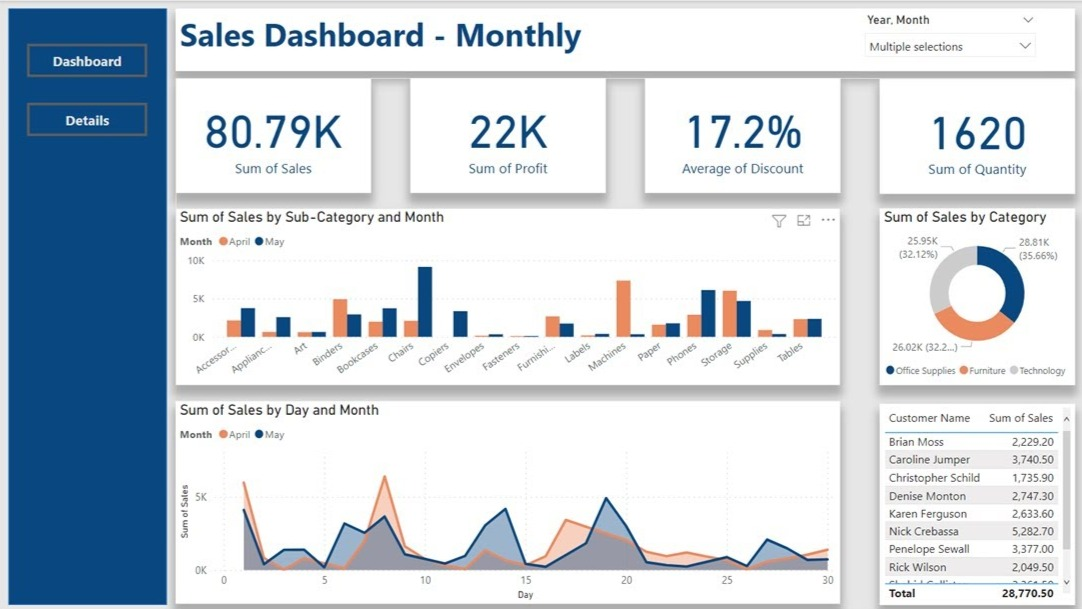
\includegraphics[width=0.9\linewidth, height=5cm]{analytical-dashboard.jpg}
    \caption{Exemplo de um \textit{dashboard} analítico}
    \label{fig:anal-dash}
  \end{subfigure}
  
  \caption{Diferentes tipos de \textit{Dashbaords}}
  \label{fig:image2}
\end{figure}

\subsection{Ferramentas para Desenho de DS ou de UI} % (fold)
\label{sub:ferramentas}

Atualmente, existem várias ferramentas para ajudar no desenho de \textit{dashboards} e interfaces de utilizador. Estas ferramentas tornam-se essenciais uma vez que permitem que a prototipagem e design deste tipo de interfaces se torne uma tarefa de fácil implementação. O desenho de interfaces de forma manual pode ser uma tarefa ineficiente e demorada, uma vez que se torna díficil de garantir a consistência visual, dificultando a interação por parte dos utilizadores. Para além de facilitar a sua implementação, o uso deste tipo de ferramentas trás inúmeras vantagem no que toca a eficiência e produtividade, ao serem utilizados elementos e estruturas já pré-definidas para facilitar a montagem e design deste tipo de interfaces gráficas.

\subsubsection{Figma} % (fold) 
\label{ssub:figma}

O \textbf{\textit{Figma}} \cite{figma} é uma ferramenta de desenho de interfaces de utilizador criada em 2012 com o principal intuito de resolver as limitações impostas pelas ferramentas tradicionais de design, sendo estas apenas ferramentas de \textit{software} com instalação e armazenamento local, impossibilitando a possibilidade de colaboração remota. O Figma é então uma ferramenta "\textit{cloud-based}", muito usada no que toca o design de interfaces e prototipagem interativa. Esta ferramenta é bastante utilizada a nível empresarial e escolar uma vez que, permite a colaboração conjunta de diferentes utilizadores num mesmo projeto de forma simultânea. O Figma é uma ferramenta cujo foco principal é a criação de interfaces, através da utilização de elementos de design já desenvolvidos, facilitando a implementação de interfaces mais complexas. A nível de interatividade, ao apresentar um design centralizado no utilizador, isto é, um design simples que não sobrecarrega o utilizador com informação desnecessária, torna a que a sua utilização e implementação de interfaces se torne numa tarefa de fácil execução. Ao apresentar também uma abordagem \textit{drag and drop}, é dado ao utilizador um sentimento de controlo e personalização maior, o que torna a implementação das diferentes interfaces mais eficiente e interativa.  %CITAR FIGMA

\subsubsection{Microsoft Power BI} % (fold)
\label{ssub:microsoft}

O \textbf{\textit{Power BI}} \cite{powerBI} é uma ferramenta de \textit{business intelligence} criada pela \textit{Microsoft}. Inicialmente esta ferramenta foi desenvolvida como uma extensão do \textit{Excel}, ajudando os utilizadores a analisar e visualizar informação de forma intuitiva. O \textit{Power BI} foi criado de forma a que os seus utilizadores pudessem criar relatórios e visualizações interativas através da transformação de grandes volumes de dados sem necessidade de programação por parte dos utilizadores, oferecendo a possibilidade de explorar os dados através de técnicas filtragem personalizadas com o uso de parâmetros definidos pelos utilizadores para que as visualizações estejam direcionadas com os interesses impostos pelos mesmos. Esta conversão dos dados é feita através de um motor de tranformação \textit{Power Query}, uma ferramente integrada no \textit{Power BI} que permite a importação e tranformação dos dados apresentados sem necessidade de programação. O \textit{Power BI} é uma ferramenta com um design bastante intuitivo e de fácil utilização, através de técnicas como \textit{drag and drop} para ajudar o utilizador no processo de criação de visualizações. Uma funcionalidade característica desta ferramenta é a possibilidade de compartilhamento de ficheiros e relatórios com outros utilizadores através da combinação do \textit{Power BI Service} e \textit{Power BI Desktop}. Esta partilha de ficheiros e relatórios permite que os utilizadores possam trabalhar de forma remota num mesmo projeto. %CITAR POWER BI

\subsubsection{Google Data Studio} % (fold)
\label{ssub:google}

O \textbf{\textit{Google Data Studio}} \cite{googleStudio}, mais conhecido como \textit{Looker Studio}, é uma ferramenta criada pela \textit{Google} com o principal intuito de criar relatórios e visualizações de dados sem necessidade de programação. Ao apresentar uma interface bastante simplista e estruturada, a sua utilização torna-se uma tarefa de fácil execução, sem grande esforço por parte do utilizador. A ferramenta apresenta uma abordagem \textit{drag and drop}, dando a possibilidade de o utilizador personalizar as diferentes visualizações e conjuntos de dados, de forma a que os mesmo se enquadrem com objetivos impostos. A nível de intertaividade, o \textit{Looker Studio} oferece ao utilizador diferentes filtros de personalização da informação e controlo de período, tornando os dados mais flexiveis de forma a responder às necessidades dos utilizadores. Por ser uma ferramenta \textit{Google}, a importação dos dados pode ser feita através de outras ferramentas já existentes como o \textit{Google Analytics}, \textit{Google Ads}, e \textit{Youtube}, desta forma, deixa de ser necessário a constante atualização manual dos dados, estando os mesmos sempre atualizados quando surgem alterações. Para além desta ferramentas, o \textit{Looker Studio} tem acesso a grandes bancos de dados, incluindo \textit{BigQuery}, \textit{MySQL}, e \textit{PostgreSQL}, permitindo os utilizadores importarem informação de diferentes fontes confiáveis de informação. O \textit{Looker Studio} ao ser uma ferramenta \textit{cloud-based}, é bastante utilizada a nível empresarial, uma vez que é permitida a colaboração simultânea dos diferentes utilizadores.

\subsubsection{Tableau} % (fold)
\label{ssub:tableau}

O \textbf{\textit{Tableau}} \cite{tableau} é uma ferramenta altamente utilizada e conhecida no mundo da visualização e criação de interfaces visuais, sendo dividida entre vários softwares, nomeadamente \textit{Tableau Prep}, \textit{Tableau Desktop} e \textit{Tableau Mobile}.

O \textit{Tableau Prep}, de forma semelhante ao \textit{Power Query} do \textit{Power BI}, é uma ferramenta cujo principal objetivo é a filtragem e limpeza dos dados. Esta ferramenta fornece ao utilizador uma imagem completa dos dados a analisar, de forma a que possa ser efetuada a sua limpeza e tranformação antes de serem utilizadas nas visualizações. Esta ferramenta encontr-se conectada com múltiplas fontes de dados tais como \textit{Excel}, \textit{SQL}, e \textit{BigQuery}, permitindo a importação de dados de diferentes fontes de informação. Com a ajuda do \textit{Hyper Engine}, o \textit{Tableau Prep} permite a que esta importação de dados seja feita de forma eficiente, não prejudicando a performance do sistema.

O \textit{Tableau Desktop} é uma ferramenta desenvolvida para facilitar a análise e a visualização de dados através da criação de dashboards interativos. Esta ferramenta tem como objetivo permitir que diferentes utilizadores de diferentes áreas consigam analisar grandes volumes de dados através de visualizações interativas sem ser necessário programar para o fazer. Através da sua interfaces gráfica simplista, e com uma abordagem \textit{drag and drop}, torna a criação de visualizações e relatórios uma tarefa de fácil execução, permitindo a integração de diferentes fontes de informação tais como \textit{Excel}, \textit{SQL Server}, e \textit{Google BigQuery}. Esta ferramenta utiliza técnologias como \textit{VizQl (Visual Query Language)} que faz a conversão direta dos dados em visualizações, permitindo uma análise mais rápida e intuitiva. Com a coloboração do \textit{Tableau Online}, é possível os diferentes utilizadores trabalharem de forma simultânea num mesmo projeto, sem a necessidade de instalação de um \textit{software} adicional, podendo também efetuar a partilha de documentos e visualizações entre os diferentes orgãos na mesma organização.

O \textit{Tableau Mobile} é uma aplicação desenvolvida para permitir a visualização de dashboards e relatórios em dispositivos móvies, tais como smartphones e tablets. Com o suporte de notificaações e alertas, os utilizadores podem ser notificados sempre que ocorram alterações nos dados ou visualizações, mantendo-se sempre atualizados.

\subsubsection{Qlik Sense} % (fold)
\label{ssub:qlik}

O \textbf{\textit{Qlik Sense}} \cite{qlik} é uma ferramenta que permite explorar e visualizar dados de forma intuitiva e interativa. Esta ferramenta possui uma ferramenta chamada \textit{Qlik cognitive engine} onde através da sua utilização são facilitadas a descobertas de relações entre os diferentes conjuntos de dados no sistema. Ao possuir uma interface \textit{drag and drop}, é permitida a criação de \textit{dashboards} personalizados sem haver necessidade de programação, facilitando a integração de utilizadores não experientes na área de visualização. O \textit{Qlik} combina inteligência artificial com a intuição humana para ajudar os seus utilizadores a descobrir padrões e tendências nos dados, facilitando a análise e interpretação da informação presente. Esta interação também é suportada através de técnicas de interação como \textit{drill-down}, \textit{filtering} e \textit{highlighting}, facilitando a navegação do utilizador nas \textit{dashbaords} em análise. 

\subsection{Recomendações para o Design de Dashboards} % (fold)
\label{sub:recomendacoes}

Aqui é onde eu vou citar os 10 principios para construir um dashboard de forma eficaz

Aqui secalhar em vez de listar mesmo os 10 principios, posso no capitulo logo inicial mencionar alguns dos principios e citar

\section{Design de Interfaces de Utilizador (UI Design)} % (fold)
\label{sec:ui_design}

Uma interface estabelece o ponto de contacto entre o utilizador e o sistema, sendo esta a principal responsável pela forma como os utilizadores interagem com o sistema. O design de interfaces de utilizador é considerado o elemento mais importante de um sistema de visualização de informação, uma vez que este design possui um impacto direto na forma como os utilizadores iram comunicar com o sistema, podendo esta interação ser pobre, resultando numa má análise de informação e num esforço cognitivo para realizar as tarefas propostas por parte do utilizador, ou ser uma implementação bastante rica e simplista, ao apresentar um design orientado para o público-alvo, nunca dificultando as tarefas a realizar pelo utilizador. De forma a criarmos um design orientado para o público-alvo que queremos atingir, Sridevi implementou três regras de "ouro" indispensáveis no que toca a implementação de interfaces de utilizador. \cite{sridevi2014user}.

\begin{enumerate}
  \item O utilizador deve estar sempre no controlo.
  \item A interface deve fazer com que os utilizadores tenham um esforço cognitivo mínimo.
  \item A interface deve ser o mais consistente possível.
\end{enumerate}

Relativamente ao ponto 1, quando é feita uma entrevista ao utilizador sobre quais os objetivos e respostas que pretendem ver resolvidos com o uso da interface, muitos utilizadores referem a necessidade de terem controlo sobre a interface, ou seja, serem eles a controlar o computador e não o computador a controlá-los. Muitas vezes o design deste tipo de interfaces limita as ações dos utilizadores devido a restrições impostas pelo \textit{designer} da interface, o que por vezes torna a interface fácil mas frustrante de utilizar. Desta forma, definir modos de interação que não influenciem os utilizadores a tomar decisões erradas ou indesejadas é crucial para o sucesso da interface. Os utilizadores devem ter a capacidade de interromper ações a meio da sua implementação, ou voltar a um estado anterior. O utilizador deve ter a possibilidade de voltar atrás nas suas decisões através de técnicas como \textit{undo} não limita as ações dos utilizadores dando lhes a possibilidade de emendar erros que possam ter surgido durante a interação com a interface. Por vezes, os utilizadores encontram-se a realizar a mesma sequência de ações vezes sem conta, pelo que a implementaçãao de 'macros' surge para facilitar estas interações recorrentes. As interfaces devem ser desenhadas de forma a que o utilizador tenha a capacidade de perceber o resultado das suas ações \cite{sridevi2014user}.

No âmbito do ponto 2, uma interface que exija que o utilizador se lembre e recorde das ações que necessita de tomar para realizar determinada tarefa não pode ser considerada uma interface bem implementada. É um facto que um utilizador tem tendência a errar mais quando se tenta lembrar de informações e técnicas necessárias para realizar determinada tarefa, uma interface bem implementada exije que as ações que os utilizadores pretendem executar sejam realizadas de forma clara, sem haver um esforço a nível cognitivo por parte dos utilizadores, guiando o utilizador a tomar as decisões corretas de forma natural. Desta forma, esta abordagem foca-se em minimizar ao máximo o esforço que o utilizador necessita de realizar para implementar as tarefas propostas, garantindo que os utilizadores não necessitem de memorizar informações e ações complexas no sistema. Quando é pedido aos utilizadores para realizarem tarefas mais complexas, é muitas vezes necessário que o mesmo uso da sua memória a curto prazo, um bom design deve facilitar a implementação destas tarefas através de sugestões ou atalhos disponíveis na interface \cite{sridevi2014user}.

Relacionado com o ponto 3, a interface deve apresentar e obter a informação sempre de forma consistente. De modo a ter uma interface consistente, é necessário que toda a informação a nível visual seja organizada de acordo um padrão de design que deve ser mantido em todas as interfaces implementadas, os mecanismos de \textit{input} devem ser limitados e utilizados de forma consistente em toda a aplicação, e os mecanismos de navegação entre tarefas devem ser definidos e implementados de forma consistente. O design de uma interface só deve ser alterado caso exista um motivo de extrema importância, uma vez que mudar o design e consistência de uma interface implica que o utilizador tenha de a reaprender \cite{sridevi2014user}.

\subsection{Recomendações para o Design de Interfaces} % (fold)
\label{sub:recomendacoes}

O design de interfaces de utilizador pode se tornar uma tarefa complexas se não forem considerados fatores essenciais e cruciais para o bom funcionamento da mesma. De forma a que o design de interfaces seja eficiente e \textit{user-friendly}, é necessário termos em consideração as seguintes 10 pr+aticas para construir \textit{dashboards} eficazes

%Principios Gerais de Design de Dashboards
%Design Visual
%Design Centralizado no Utilizador
%10 Best Principles for Building Effective Dashboards

\subsection{Metodologias para o Design de Interfaces} % (fold)
\label{sub:metodologias}

Dizer que nesta secção a pproach que irei ter vai ser segundo essas 3 possibilidades de implementação de design de interfaces

%Modelo GQM (Goal-Question-Measurement)
%Processo Iterativo no design de Dashboards
%Design Informado por Dados


\section{IVML}
\label{sec:ivml}

%Ainda não sei o que e que vou falar aqui, ver secalhar depois com os professores

\section{IVML Designer}
\label{sec:ivml_designer}

%Aqui é onde vou meter os diagramas de classes que tive a desenvolver em detalhe

%Secalhar (falar com os professores) posso também meter os laayouts que eu fiz a simular a aplicação a explicar o que é que eu quero que a aplicação faça e como é que quero que ela se comporte
